% Compilar com: pdflatex DADOS_ALERTARIO_RADAR_SUMARE_PIBIC.tex
\documentclass[11pt,a4paper]{article}
\usepackage[T1]{fontenc}
\usepackage[utf8]{inputenc}
\usepackage[brazil]{babel}
\usepackage{geometry}
\usepackage{booktabs}
\usepackage{graphicx}
\usepackage{hyperref}
\geometry{margin=2.5cm}
\graphicspath{{./figures/}{docs/figures/}}
\hypersetup{colorlinks=true,linkcolor=black,urlcolor=blue}
\setlength{\parskip}{0.55em}
\setlength{\parindent}{0pt}
\title{Dados do Sistema Alerta Rio e do Radar Meteorológico do Sumaré\\\large Nota técnica para o relatório PIBIC}
\author{Projeto RioNowcast}
\date{28 de setembro de 2026}
\begin{document}
\maketitle

\section{Objetivo e escopo}
Este documento descreve os dados empregados na versão auditável do dataset para nowcasting de precipitação no município do Rio de Janeiro. O dataset combina imagens históricas do radar meteorológico do Sumaré e observações pluviométricas das estações do Sistema Alerta Rio, no período 2012--2024. A versão processada é \texttt{radar\_sumare\_2012\_2024\_15min\_128\_audited\_v3}.

O objetivo do processamento não é estimar uma grandeza física de refletividade a partir de uma imagem colorida. Ele produz uma representação auditável do produto visual do radar, temporalmente alinhada às medidas de chuva das estações, para experimentos comparativos de nowcasting.

\section{Estações pluviométricas do Alerta Rio}
As séries históricas originais do Alerta Rio fornecem acumulados de chuva em milímetros por intervalo de 15 minutos (mm/15 min), identificados no pipeline como \texttt{m15}. Assim, valores e métricas devem ser reportados em mm/15 min; uma interpretação em mm/h requer conversão explícita.

O timestamp \texttt{m15} representa o \emph{fim} do intervalo acumulado. Para associá-lo a uma janela de radar indexada pelo início, aplica-se deslocamento de $-15$ minutos. Valores ausentes não são imputados: uma máscara indica pixels e instantes observados, e ausências não participam da função de perda nem das métricas.

O mapeamento espacial versionado contém 33 estações. A auditoria dos targets esparsos nos 13 anos confirmou 33 coordenadas presentes, 33 coordenadas compatíveis com o mapeamento e nenhuma coordenada esparsa sem correspondência. Identificadores eventualmente presentes nas séries brutas não foram usados sem coordenada validada no domínio do radar.

A geração dos targets processou 12\,332\,637 registros estação--tempo entre 2012 e 2024. Os targets são armazenados de forma esparsa, pois somente pixels de estações possuem observação pluviométrica.

\section{Radar meteorológico do Sumaré}
O radar do Sumaré é um radar banda C operado pelo Sistema Alerta Rio. O acervo disponível neste estudo contém imagens PPI em PNG, capturadas aproximadamente a cada dois minutos. O arquivo numérico original de PPI ou de refletividade não foi armazenado. Portanto, o pipeline usa exclusivamente a informação RGB do produto de imagem.

As imagens históricas possuem 656 colunas por 654 linhas, quatro canais (RGBA), e já contêm apenas o bitmap de refletividade; não há legenda lateral a recortar nesse arquivo. O centro adotado do radar é $22^\circ57'18{,}5''$ S, $43^\circ14'53{,}8''$ W, a 695,51 m de altitude. O raio operacional usado no georreferenciamento é 138,9 km, informado pela operação do sistema. Isso corresponde aproximadamente a 425 m por pixel na imagem original e a células de cerca de 2,17 km de lado (4,7 km$^2$) no produto reamostrado de 128 $\times$ 128. Estes são valores geométricos aproximados, não uma grade cartográfica oficial.

Os nomes dos PNGs representam hora local de \texttt{America/Sao\_Paulo}. O pipeline converte timestamps para UTC, inclusive nos períodos históricos de horário de verão. Para cada janela de 15 minutos, exige-se no mínimo seis imagens. A agregação \texttt{rgb-max} usa o máximo canal a canal entre imagens válidas, e o resultado é reamostrado por vizinho mais próximo para 128 $\times$ 128.

\textbf{Limitação:} \texttt{rgb-max} preserva uma convenção visual compatível com o pipeline legado, mas não é agregação física de refletividade nem conversão de RGB para taxa de chuva. Uma calibração da paleta ou acesso a campos quantitativos constitui trabalho futuro.

\subsection{Frames ilustrativos}
A Figura~\ref{fig:radar-frames} apresenta dois frames históricos selecionados entre eventos com chuva observada nas estações. As cores correspondem ao produto RGB disponibilizado pelo radar; elas não devem ser interpretadas como valores quantitativos calibrados de refletividade ou taxa de precipitação. O sufixo \texttt{m15} indica o maior acumulado de 15 minutos observado entre as estações no evento selecionado.

\begin{figure}[htbp]
\centering
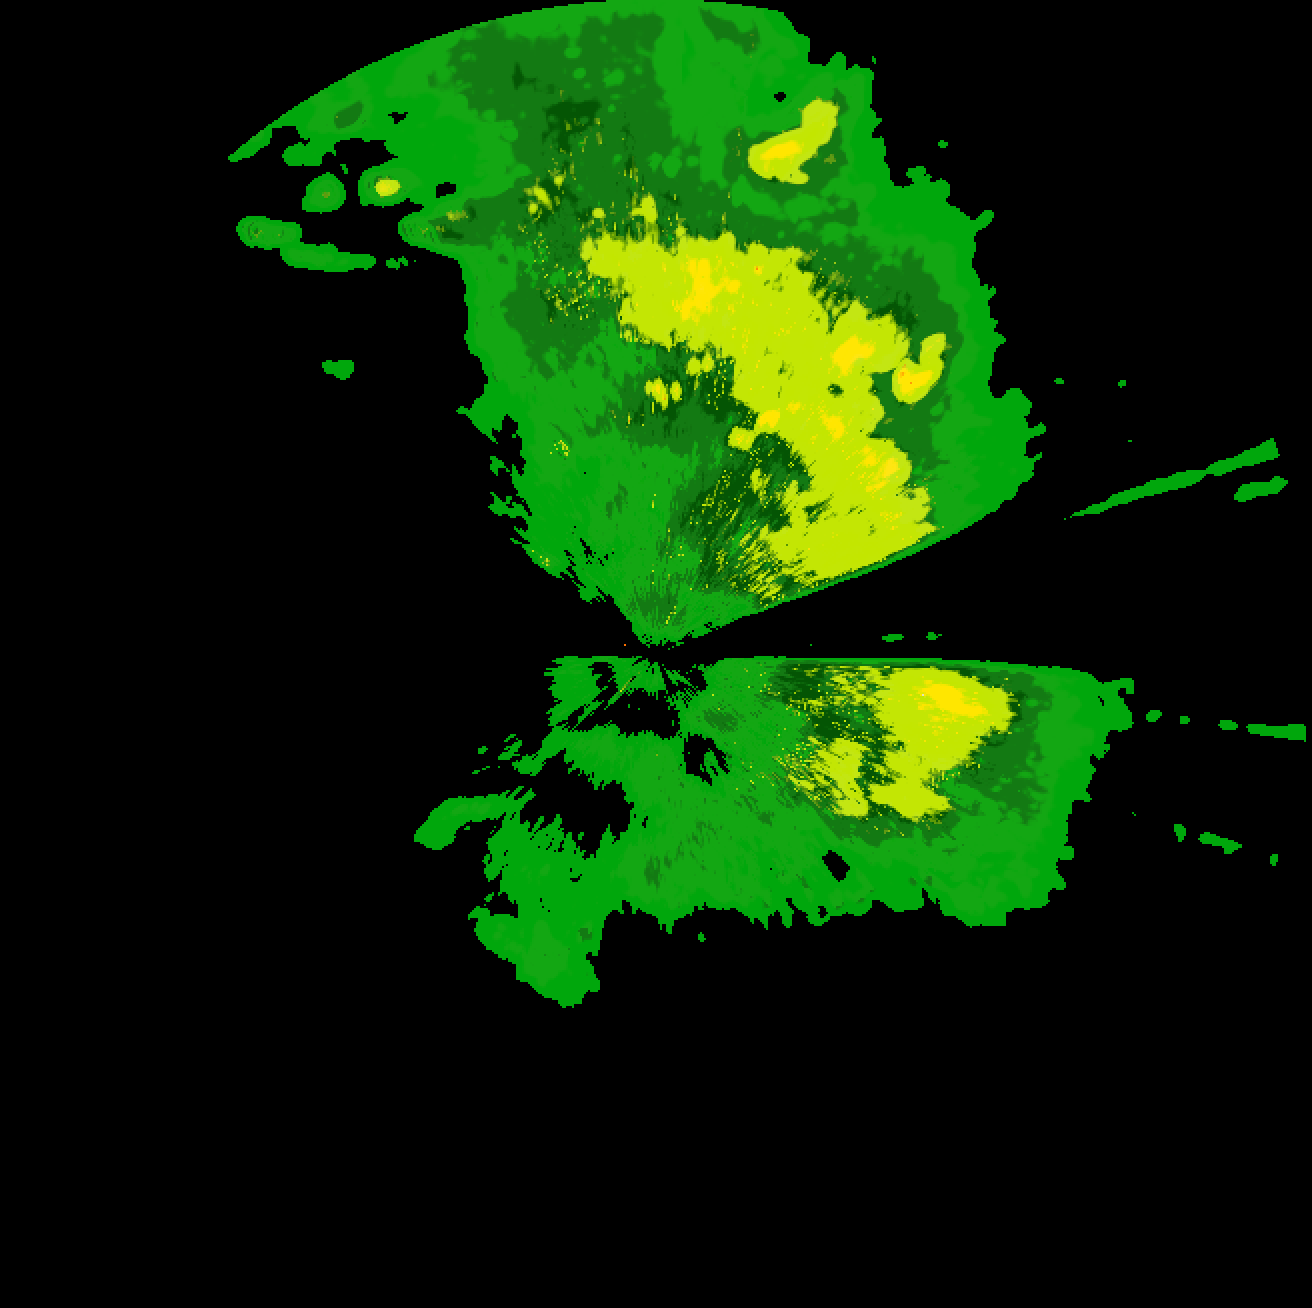
\includegraphics[width=0.47\textwidth]{radar_sumare_20230330T2215_m15_39.80.png}
\hfill
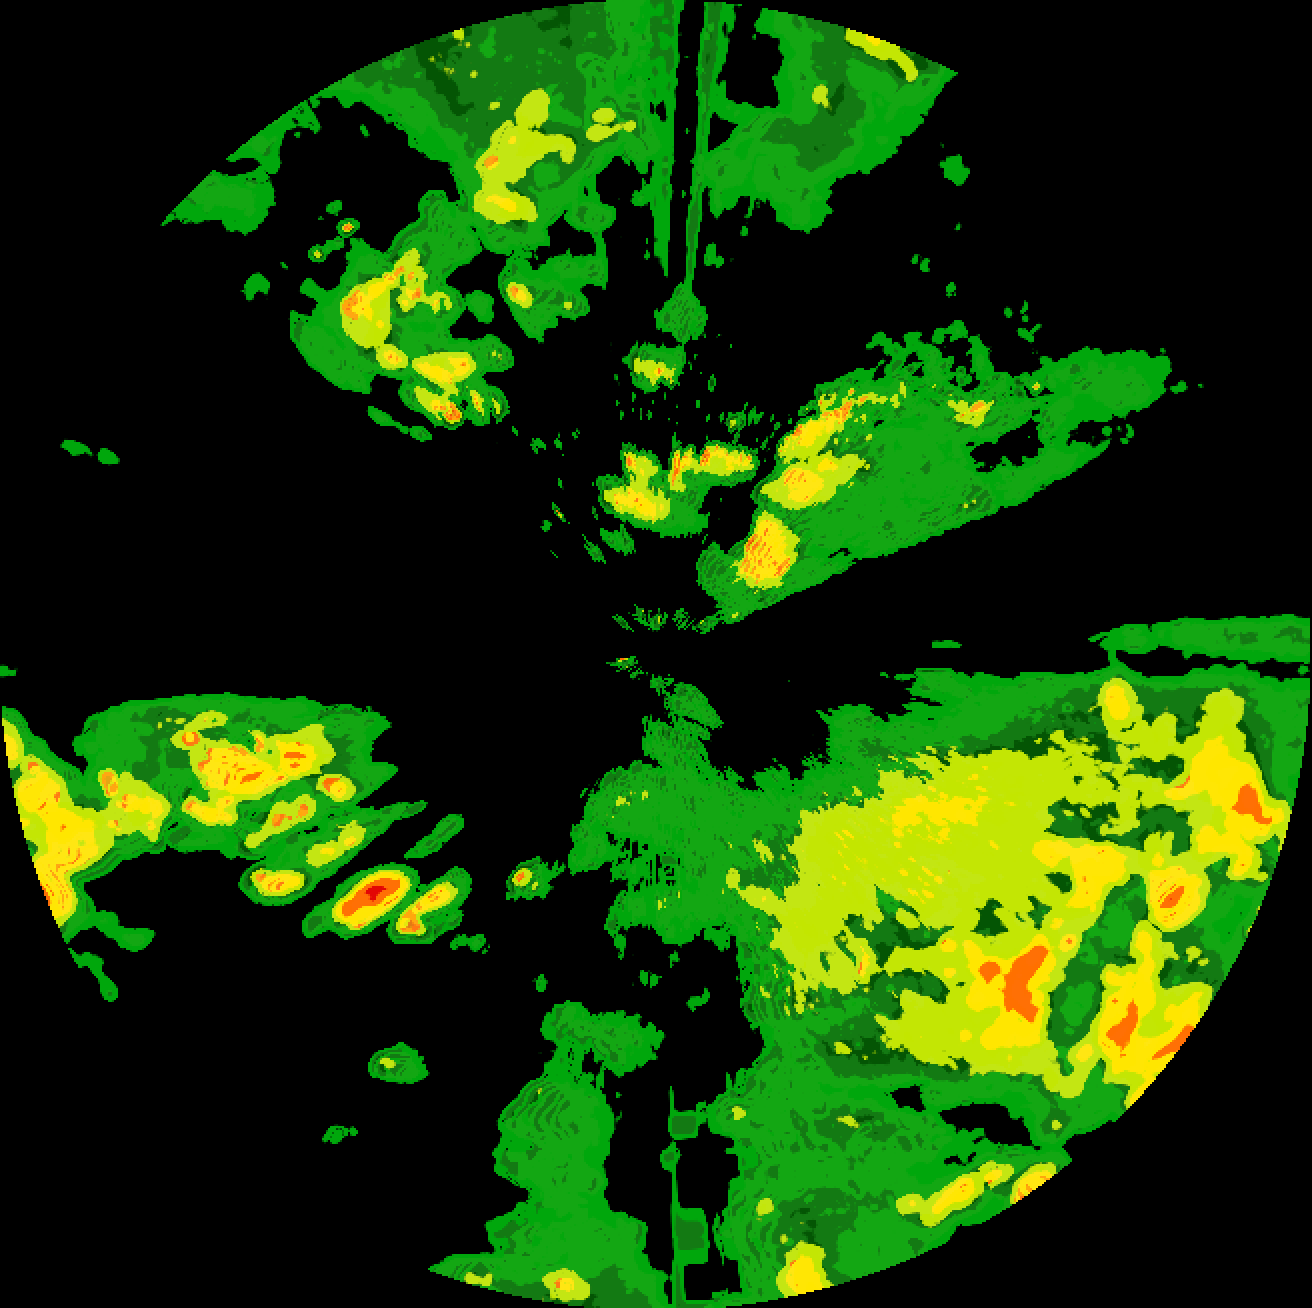
\includegraphics[width=0.47\textwidth]{radar_sumare_20241220T1930_m15_35.40.png}
\caption{Frames PPI RGB do radar do Sumaré associados a eventos chuvosos: à esquerda, 30 de março de 2023 às 22:15 UTC (máximo observado: 39,80 mm/15 min); à direita, 20 de dezembro de 2024 às 19:30 UTC (35,40 mm/15 min).}
\label{fig:radar-frames}
\end{figure}

\section{Alinhamento espacial e temporal}
O mapeamento usa projeção azimutal equidistante esférica centrada no radar, com norte no topo da imagem e leste à direita. A hipótese \texttt{geographic\_aeqd\_north\_up} foi selecionada em auditorias independentes de 2023 e 2024. As correlações de postos entre sinal do radar e chuva foram 0,733 em 2023 e 0,689 em 2024; as diferenças entre taxas de detecção de eco em eventos chuvosos e secos foram 0,670 e 0,683, respectivamente.

O melhor alinhamento bruto entre \texttt{m15} e o nome local do PNG foi $-195$ minutos: $-180$ minutos de fuso UTC$-$3 e $-15$ minutos porque \texttt{m15} marca o fim do intervalo. No dataset final, o radar é indexado no início UTC da janela e os targets usam offset de $-15$ minutos.

\section{Cobertura e controle de qualidade}
A Tabela~\ref{tab:frames} apresenta os compósitos de 15 minutos publicados por ano. Cada janela só é publicada quando possui ao menos seis imagens válidas. O dataset possui 374\,131 compósitos e ocupa aproximadamente 18 GB.

\begin{table}[htbp]
\centering
\caption{Compósitos de radar publicados por ano.}
\label{tab:frames}
\begin{tabular}{rrrrrr}
\toprule
Ano & Frames & Ano & Frames & Ano & Frames \\
\midrule
2012 & 33\,846 & 2013 & 31\,887 & 2014 & 32\,737 \\
2015 & 29\,637 & 2016 & 31\,473 & 2017 & 28\,826 \\
2018 & 28\,725 & 2019 & 25\,527 & 2020 & 23\,317 \\
2021 & 29\,300 & 2022 & 27\,147 & 2023 & 26\,658 \\
2024 & 25\,051 & & & & \\
\bottomrule
\end{tabular}
\end{table}

O acervo bruto não tem cobertura uniforme. Em 2019, 681 das 26\,208 janelas inicialmente candidatas foram descartadas por PNGs inválidos; em 2020, foram 297 de 23\,614. A maior parte dos arquivos inválidos foi classificada como \texttt{UnidentifiedImageError}, isto é, arquivo que não pôde ser decodificado como imagem. Essas ocorrências não entram no memmap final. O loader também descarta sequências que atravessem lacunas superiores a 15 minutos.

\section{Protocolo experimental de referência}
O protocolo multianual usa 2012--2021 para treinamento, 2022 para validação e 2023--2024 para teste. Uma amostra usa cinco janelas passadas e prevê cinco futuras: 75 minutos de histórico e 75 minutos de horizonte, com stride de cinco janelas. Após o filtro de continuidade, o treinamento possui 53\,519 amostras.

As classes usam limiares de 1,25; 6,25; e 12,5 mm/15 min. A Tabela~\ref{tab:classes} evidencia o desbalanceamento: eventos fortes e extremos são raros, principalmente entre julho e outubro. Todos os meses são mantidos no dataset canônico; amostragem balanceada é uma opção experimental.

\begin{table}[htbp]
\centering
\caption{Classes nas 53\,519 amostras de treinamento.}
\label{tab:classes}
\begin{tabular}{lrr}
\toprule
Classe & Janelas & Fração \\
\midrule
Fraca ou seca & 48\,176 & 90,02\% \\
Moderada & 4\,013 & 7,50\% \\
Forte & 850 & 1,59\% \\
Extrema & 480 & 0,90\% \\
\bottomrule
\end{tabular}
\end{table}

\section{Recomendações de interpretação}
\begin{itemize}
\item Reportar erros em mm/15 min e converter para mm/h somente quando explicitamente necessário.
\item Distinguir experimentos do dataset auditável de resultados legados, que não aplicavam a convenção temporal validada.
\item Reportar resultados globais e por intensidade, pois a métrica global é dominada por situações secas ou de chuva fraca.
\item Tratar o RGB como entrada visual, não como refletividade quantitativa.
\item Manter a máscara de ausências; não substituir ausência por zero.
\end{itemize}

\section{Rastreabilidade}
Os artefatos principais são:
\begin{itemize}
\item configuração do radar: \url{configs/radar_sumare_historical_audited_v1.json};
\item mapeamento espacial: \url{configs/mapeamento_pixel_estacao_alertario_historical_v1.csv};
\item metadados anuais: \texttt{metadata.json}, \texttt{radar\_timestamps.npy} e \texttt{window\_coverage.csv};
\item targets: \texttt{targets\_alertario\_sparse.npz};
\item relatórios: \url{outputs/analysis/alertario/} e \url{outputs/analysis/radar_sumare/}.
\end{itemize}

\end{document}
